\chapter{Jupyter Notebooks}
Jupyter Notebooks are a very useful data analysis tool, especially among data scientists and Python programmers, since they allow you to run code inline with your document. There are many tools that allow you to create and edit Jupyter Notebooks, such as Google Colab or Anaconda.\par
\section{What Are Jupyter Notebooks?}
At their most basic, Jupyter Notebooks are just spicy binders. They allow you to write Python code and add notes in a quick and easy way. You'll find that Jupyter Notebooks are actually quite common in academic settings, since they allow academics to share their exact findings with each other in an organized manner. \par
Jupyter Notebooks always have the file extension \verb|.ipynb| (though the curious among you may try to open these files in a text editor to discover that they're just JSON files). IPYNB stands for Interactive PYthon NoteBook. It's not uncommon to have multiple notebooks, although some people choose to pile everything into one notebook.\par

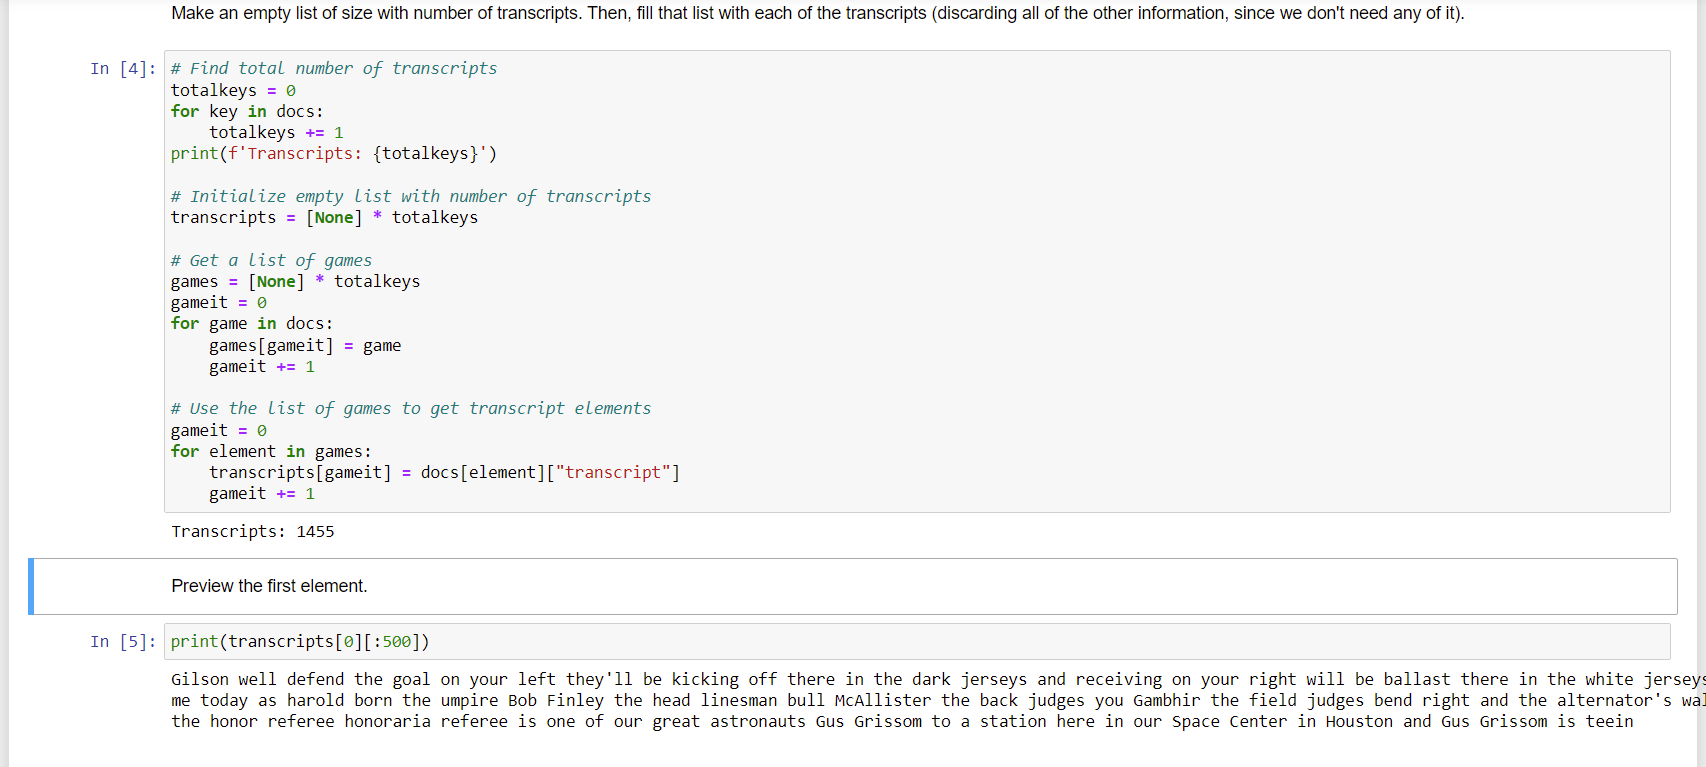
\includegraphics[width=0.8\textwidth]{img/jupyternotebook.png}

When you're writing in a Jupyter Notebook, you can either write in a markdown block or a code block. Your markdown code will only be rendered, not executed. Even if you specify that a chunk of code should have its syntax highlighting in Python, it will not be executable. Essentially, your markdown code is read-only. However, your code blocks are read/write/executable. You can execute any of the Python code inside of a dedicated Jupyter Notebook code block.\par
\section{Basic Markdown Syntax}
Jupyter Notebooks support standard markdown syntax, such as what you might use on an Internet forum or on GitHub in \verb|.md| files (like READMEs or Contributing files). If you've never worked with markdown before, it's not too difficult. Markdown is just a way to change the appearance of plain-text while writing in plaintext. When writing markdown, you'll typically write it in a plain-text form, then open the same document in a markdown renderer. When you're working with Jupyter Notebooks, your notebook will be your markdown renderer.\par
The most basic of the markdowns is paragraph text. Paragraph text is written with no extra or special symbols.
\begin{lstlisting}
This is just regular paragraph text.
\end{lstlisting}

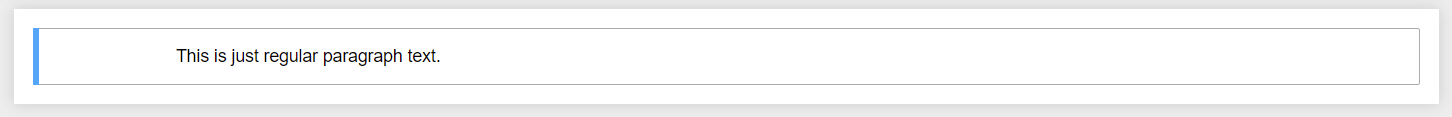
\includegraphics[width=0.8\textwidth]{img/mdparagraph.png}

You can add additional emphasis styling to your paragraph text, just like you would in any other word processor: italics and bold. To italicize something, use single asterisks to mark the beginning and end of the italicized area. To bold something, use double asterisks to mark the beginning and end of the bolded area. You can also use combinations of asterisks to denote both italicized and bolded text. To create a line break, add an extra blank line, as a single line break won't add an extra line. Your symbols cannot span multiple lines, so if you want more than one line to be emphasized, you need to write more than one set of symbols for the respective emphasis symbol sequence.\par
\begin{lstlisting}
This is *italicized* and **bold**.

This is ***italicized and bold***.
\end{lstlisting}
\par

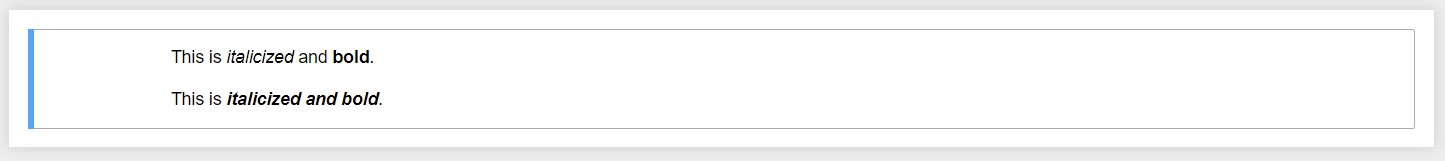
\includegraphics[width=0.8\textwidth]{img/mditalicbold.png}

Another common block to use is writing snippits of code. This is different from writing code in a Jupyter Notebook code block. Code in a markdown block cannot be run; only code in code blocks can be run. You can choose the syntax highlighting that is used when writing in a code block. To write in a code block, use three backticks to mark the beginning and end of your code block. To write inline code, use single backticks.\par
\boxtext{Where's the backtick?}{The backtick is the character right next to the number 1 key on most US-layout ANSI and ISO keyboards. Shift-Backtick normally gives you tilde \string~.}
\begin{lstlisting}
This is some inline code: `print()`

```
# No syntax highlighting
print("Hello, world!")
print("This is Python!")
```

```python
# Python syntax highlighting
print("Hello, world!")
```

```cpp
# C++ syntax highlighting
std::cout << "Hello, World!" << endl;
std::cout << "This is C++!" << endl;
```
\end{lstlisting}
This is some inline code: \verb|print()|
\\
\begin{lstlisting}
# No syntax highlighting
print("Hello, world!")
print("This is Python!")
\end{lstlisting}
\begin{lstlisting}[style=pippython]
# Python syntax highlighting
print("Hello, world!")
\end{lstlisting}

\begin{lstlisting}[style=cpp]
// C++ syntax highlighting
std::cout << "Hello, World!" << endl;
std::cout << "This is C++!" << endl;
\end{lstlisting}
\footnote{These colors have been simulated.}The exact coloring and style of your Jupyter Notebook code will depend on the renderer that you're using.\par
At the top of your project and to divide each of the subsections, you might want to include a header. There are six header sizes, which are determined by how many \verb|#| symbols are added before your heading text.
\begin{lstlisting}
# The largest heading
## The second largest heading
###### The smallest heading
\end{lstlisting}
You can also include links in your code. To create a hyperlink, wrap the link text in brackets \verb|[]| followed by the URL in parentheses \verb|()|.\par
\begin{lstlisting}
We're writing code in [Python](https://www.python.org/).
\end{lstlisting}

The best way to get to know how to use and write markdown is to just write more text in markdown. Before long, it will become second nature!\par
\section{The Interactive Python Shell}
Let's get to the "interactive" part of IPYNBs. The killer feature of Jupyter Notebooks is their ability to run code inline. Jupyter Notebooks that are opened in compatible software actually have their own Python interpreter that can run Python code, including loading modules and reading files.\par
In order to use this interpreter, you need to add a code block to your Jupyter Notebook. Every piece of software has a different way of doing this, but once you've gotten your code block in your notebook, you can then write any Python code inside of that block. One of the really cool things about Jupyter Notebooks is your ability to create multiple code blocks in one notebook. Even when you have multiple code blocks, your notebook will still keep all of the variables and states that you created in earlier blocks. For example, let's say that you created a variable first thing in your Jupyter Notebook. Then, three code blocks later, you decide that you need to use that variable. The variable is still active until the Jupyter Notebook Python runtime is reset or the notebook is closed.\par
Once you've written your code in a Jupyter Notebook, you can run it by either using a keyboard combination (typically Shift + Enter) or by pressing the Start button on the left side of the code block. Once the code block has finished its execution, you'll be able to use any of the variables that you've declared in future code blocks.\par
When you are running code in a Jupyter Notebook, it is entirely likely that you will make a mistake when writing your code. You might accidentally make an infinite loop, or perhaps your program isn't asking for user input correctly. In these cases, it is important to know how to \newterm[interrupt]{interrupt} the flow of your program. In the console, the easiest way to send an interrupt (specifically, a \newterm[KeyboardInterrupt]{interrupt}) is to press Ctrl+C on the keyboard. This interrupt was designed to be send by a keyboard during the DOS computer days (and before), when the keyboard was the only method a programmer had of interrupting the execution of a program. In fact, modern "stop" buttons simply emulate a Ctrl+C in the IDE. 